\chapter{Reinforcement Learning}
%\chapter{Reinforcement Learning}
In this chapter I will introduce the notions and notations
used in reinforcement learning.

\section{Reinforcement Learning Framework}
There are only few components to the reinforcement learning problem.
The learner and actor is dubbed the agent and everything outside it the environment.
The agent perceives its environment and acts on it,
receiving a reward in return.
The latter is a numerical value
which the agent tries to gain as much as possible of
during its time interacting with the environment.
This interaction goes on continually:
observation followed by action followed by reward.
The goal of the agent is to maximize its accumulated reward
over the entire span of a task,
i.e. an instance of a problem.
In order for it to do so
it must learn to not only look to immediate rewards
but must also look to what the future has to offer.

\begin{figure}[h]
	\center
	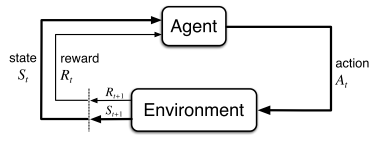
\includegraphics[width=.5 \linewidth]{agent-environment.png}
	\caption{The agent interacts with the environment and consequentially perceives a reward and the next state of the environment.}
	\label{agent-env}
\end{figure}

Formally, we divide the problem into discrete time steps $t$.
A time step occurs every time the agent perceives a state $s_t$
from the set of possible states $\mathcal{S}$.
Based on this state the agent selects an action $a_t$
from its repertoire of actions $\mathcal{A}(s_t)$
available to it at in state $s_t$.
As a result, the next step it will receive a numerical reward $r_{t+1}$
along with the next state $s_{t+1}$,
and so on and so on.

As you can see, the problem setting is entirely abstract
and can be filled in in various ways.
In fact, the same practical problem may be defined in different ways
depending on the goal.
A state could just as well represent a robot's raw sensor readings
as well as higher-level representations
such as whether it's looking at a green or red light.
We say that state is provided by the environment
even though one could argue a robot's sensors
are part of the agent.
Instead, we look at the agent as the observer and decision-maker
taking in everything from a distance,
even its physical body external to it
as part of the environment.
Similarly to states,
actions can range from raw low-level values
like motor voltages
to higher-level concepts like which room to go to
or whether to turn left or right.
Basically, actions are decisions taken by the distant observer,
for the designer to decide which shape they take.

\section{Markov Decision Processes}
The Markov property is an interesting property for a problem to have
because it states that all relevant information at some point
is present in a state.
This means that the whole history leading up to a certain point,
insofar that it is relevant,
is encoded in the state at that time. 
Such a state is said to be Markov.

Formally, consider the probability of ending up in a state $s_{t+1}$
with reward $r_{t+1}$
after performing some action $a_t$
in a state $s_t$.
This probability is denoted

$$Pr(s_{t+1}=s', r_{t+1}=r | s_t, a_t)$$

We would say a state signal is Markov if this probability is the same as

$$Pr(s_{t+1}=s', r_{t+1}=r | s_t, a_t, s_{t-1}, a_{t-1},..., s_0, a_0)$$

which is the same scenario except given the entire state and action history. If these two are indeed equal, then the history is effectively encoded in the current state $s_t$.

\paragraph{}
START on mdp's here

\section{Value Functions}

\section{Temporal Difference Learning}

\section{Q-Learning}
Often we will discount future rewards
by a certain factor $\gamma$ per time step,
resulting in a total future discounted return
for the agent of
$R_t = \sum{T}{t'=t} \gamma^{t'-t}r_{t'}$,
with T the last time step.
This return is dependent on some policy $\pi$.
We now define $Q*(s,a)$ as the maximum expected return
when in a state s and taking action a.
This assumes we already know the optimal policy
in every subsequent state.
More formally,
$Q*(s,a) = max_{\pi}E[R_t|s_t=s, a_t=a, \pi]$

\paragraph{}
Since we assume we already know the optimal action in every state,
$$Q*(s,a) = E_{s'~\mathcal{E}}[r+\gamma max_{a'}Q*(s',a')|s,a]$$

Q-learning uses this equation directly
by plugging it into an iterative update.
Every step, the known Q-value for the visited state-action pair
is updated using a simple update rule:

$$<<TODO Q-learning update rule>>$$

with $\alpha$ a discount factor to stabilize the update.
This learned action	-value function directly approaches
the optimal action-value function $Q*$,
meaning that it always learns the optimal policy
of taking action $a' = argmax_{a}Q(s,a)$
in any state s.
The policy that is used to learn these Q-values
is only used for exploration purposes such that
sufficient state-action pairs are visited
and updated.
However, the policy itself is not optimized.
We call this off-policy learning,
as opposed to on-policy learning such as Sarsa-TD
where Q-values are updated with respect to
the currently used policy.
An advantage of Q-learning
is that it is guaranteed to converge
with probability 1
once certain conditions are fulfilled,
such as sufficiently small step size $\alpha$.

\paragraph{}
A problem with this learning approach is that
it enumerates all state-action pairs,
without generalization beyond visited pairs
and the added disadvantage of having to visit
each state-action pair multiple times
in order to have the Q-values converge.
Note that this makes the exploration strategy especially important,
as an agent that starts with a default Q-value assumption of 0
for each state-action pair can easily overfit
to non-zero Q-values if it is too greedy.
Moreover, and most importantly,
this approach does not scale well beyond only the smallest and most trivial
of state-action spaces.
This because the agent won't be able to enumerate all state-action pairs
sufficiently in such scenarios.
In the next section I will discuss how to alleviate this problem.

\section{Function Approximation}
To combat the problems brought along by a large state-action space,
we can use function approximators instead of storing Q-values
for each state-action pair,
which would quickly become infeasible.
To this end,
we could use any approximation method commonly used in machine learning
to approximate our state-action values.
However, reinforcement learning makes some methods
less suitable than others.
Samples gathered iteratively using reinforcement learning
usually have high correlation since an agent
takes a certain path through
the state-action space,
where neighboring states are usually somewhat similar.
The target to be learned is also not stationary,
since the real target value is often now known
but bootstrapped with some estimation.
For example,
in Q-learning the optimal action-value function $Q*$
is approximated using $r+\gamma max_{a'}Q(s',a')$
since we do not know the optimal $Q*$ in advanced.
This substituted target is still changing
because it has not been learned fully yet
and is both the value to be learned
as the target used for learning.
In subsequent sections I will discuss
how we can minimize the impact of these problems.
Still, it is important to be aware of them
when designing a function approximator.

\paragraph{}
One way of looking at the error of a Q-value approximator
with parameters $\theta$ is to look at the Mean Squared Error
between between the maximum expected return and
the predicted state-action value for all state-action pairs:
% formula kinda from sutton
% https://webdocs.cs.ualberta.ca/~sutton/book/ebook/node86.html
$$MSE(\theta) = \sum_{s \in S}[Q*(s,a)-Q(s,a,\theta)]^2$$
This error can then to be minimized over all samples
by a method such as gradient descent (discussed next)

That is the traditional machine learning approach.
Note that reaching a global optimum for the parameters
is often only possible for linear functions
and not so anymore for more complex nonlinear functions.
In the harder case, we could instead look for local optima,
i.e. a case when $MSE(\theta') < MSE(\theta)$
for all $\theta$ near $\theta'$.

One should also be careful with simply minimizing the MSE
of the state-action function approximator
as our ultimate goal is to have the best policy $\pi$,
% TODO so.. do they collide? Sutton was vague at first	
two goals that do not necessarily collide.

\subsection{Gradient Descent}
Gradient descent is a method for minimizing the error
over all examples.
It works by moving the parameters of some function approximator
in the direction that most reduces the error for some example.
Denote with $\theta$ the parameters
and with $\Delta_{theta_t}f(theta_t)$ the vector of partial derivatives
for some function f.
Then:
% Basically this one from sutton
% https://webdocs.cs.ualberta.ca/~sutton/book/ebook/node87.html
$$ \theta_{t+1} = ... $$
As a result, the step will be proportional
to the negative gradient of the example's squared error
and regulated by a parameter $\alpha$.

In fact, this is actually called
stochastic gradient descent
as the update is done after each training sample,
instead of after the whole batch
as in standard gradient descent in machine learning.

However,
we still do not have
$Q*$, meaning we have to substitute
or bootstrap it with an approximation.
If this approximation is an unbiased estimate,
$\theta_t$ is guaranteed to converge
to a local optimum
for decreasing step-size $\alpha$.

\section{Eligibility Traces}
Valt te overwegen.
